\section{Thermal resistance}
\label{sec:rth}

The thermal resistance ($\Rth$) is
the only experimentally accessible quantity
to asses the heat flow
in the structure \cite{Heinen2012}.
The thermal management
of a VECSEL is of critical importance
\cite{Tropper2006,Kemp2008,Vetter2012,Giet2008}.
Consequentially,
we're interested to determine $\Rth$.
It is a useful
figure of merit
to keep track of improvements
on design and manufacturing process
of VECSEL technology.
The thermal resistance
describes how much the sample heats up ($\d T$)
as a result of the dissipated power $\d D$
\begin{equation}
\d T = \Rth \d D \quad \Rightarrow \quad \Rth = \pd{T}{D}.
\label{eq:rth}
\end{equation}

There are several methods deployed
to determine
the thermal resistance,
an overview can be found in \cite{Heinen2012}.
Most of them are time and equipment intensive.
This is impractical
in order to monitor
improvements made in a design and
manufacturing process.
More simple approaches are desired.
For this report
I review two methods
that are supposed to be
just that.


\subsection{By spectral shift}
\label{sec:rth:lambda}

We can write the thermal resistance from (\ref{eq:rth})
as \cite{Heinen2012,Giet2008}
\begin{equation}
\Rth = \pd{T}{D} = \pd{\lambda}{D}/\pd{\lambda}{T}.
\label{eq:rth_long}
\end{equation}
In this description
$\lambda$ corresponds to
the longest emitted wavelength.
The longest emitted wavelength is said to
correspond to the hottest part of the VECSEL.
This is a result of the predominantly linear shift
in refractive index
as function of temperature \cite{Heinen2012}.
This approach ignores
the change in cavity length
resulting from thermal expansion.

The longest emitted wavelength
is correlated
with dissipated power.
This gives a linear relation
for each heat sink temperature
\begin{equation}
\lambda_{\Ths} = \left.\pd{\lambda}{D}\right|_{\Ths} D + \lambda_{0,\Ths}.
\end{equation}
By substituting
\begin{equation}
\lambda_{0,\Ths} = \pd{\lambda}{T} \Ths + \lambda_0
\end{equation}
we end up with \cite{Heinen2012}
\begin{equation}
\lambda = \pd{\lambda}{D} D + \pd{\lambda}{T} \Ths + \lambda_0,
\label{eq:rth_fit}
\end{equation}
from where we can extract
the required parameters for (\ref{eq:rth_long})
using linear regression.

We record the emitted spectrum
for every pump setting.
In order to determine
the longest emitted wavelength
we cut
these spectra
as indicated
in Fig.~\ref{img:longest_wavelength}.
By measuring each pump setting multiple times,
we can increase our confidence
in the extracted wavelength value.

\begin{figure}
\centering
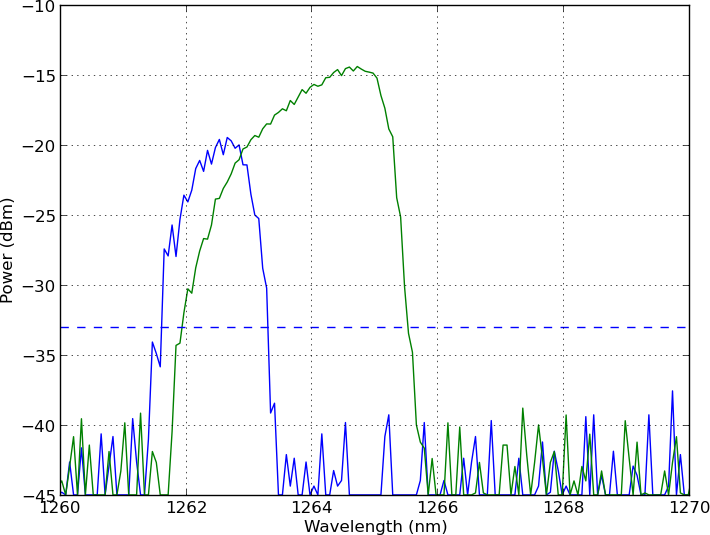
\includegraphics[width=10cm]{img/longest_wavelength.png}
\caption{We cut the spectrum
at a level
above the noise floor.
For each pump setting
we have multiple measurements,
giving us a margin
of how reliable this extracted
longest wavelength is.}
\label{img:longest_wavelength}
\end{figure}

The dissipated power $D$
corresponds to the left-over power
of the pump ($P$),
after we have accounted for the
reflected ($R$) and emitted ($E$) part
\cite{Heinen2012},
\begin{equation}
D = P - R - E.
\label{eq:dissip}
\end{equation}
\subsection{By roll over}
\label{sec:rth:trollover}

A second method,
relies on an intrinsic roll over temperature.
Roll over is an effect due to the optical pumping:
While increasing the pump power
in order to obtain higher emitted output,
we heat the gain structure.
This increase in temperature
introduces an additional loss
which the gain
has to compensate.
Otherwise,
our device stops lasing.
After a certain point
the gain cannot compensate for the losses anymore,
and this region stops contributing
to the output.
We see
a decline
in output power
despite the higher pump --
a roll-over.

Heinen et al. \cite{Heinen2012}
have found empirically --
using the method described in \ref{sec:rth:lambda} --
the longest wavelength
at this roll over point
is the same wavelength,
regardless of the heat sink temperature.
They conclude,
this wavelength to correspond
to an of the structure intrinsic
critical temperature --
the roll over temperature.
Given definition (\ref{eq:rth})
we find
the difference in temperature
between (unknown) roll over and heat sink.
It is
the thermal resistance
times the dissipated power,
\begin{equation}
T_\mathrm{ro} - \Ths = \Rth D_\mathrm{ro}.
\end{equation}
In other words,
when we plot
dissipated power at roll over ($D_\mathrm{ro}$)
versus the heat sink temperature
for this measurement $\Ths$,
we find a linear relation.
Its slope corresponds
to the thermal resistance,
and the $y$-intersection
to the roll over temperature \cite{Heinen2012}:
\begin{equation}
\Ths = -\Rth D_\mathrm{ro} + T_\mathrm{ro}.
\end{equation}

This relation is wavelength independent.
Mode instabilities in pump and emission
are expected to result in fluctuations
in the emitted spectra.
A spectrum independent method
to determine $\Rth$ is thus supposed to
yield a result with smaller uncertainty.
The difficulties in this second method
arise from identifying
the exact point of roll over.
Whether this identification
is more or less error-prone
is open for discussion.
Furthermore,
it is not yet clear
whether all VECSEL designs
show this intrinsic roll over behavior.
\subsection{Remarks on experimental access and corrections}

Hader et al. \cite{Hader2013}
have pointed out,
the used definition of
dissipated power (\ref{eq:dissip})
ignores a relevant loss channel.
Namely,
beside the reflected,
emitted,
and dissipated part
there are additional non-heating losses
the incident pump converts into.
These additional losses come from
non-heating spontaneous emission
and surface-scattering.
Without these
we overestimate $\Rth$.
The losses due to surface-scattering
are particularly pronounced
when using an output coupler
with low out-coupling losses.

From a theoretical point of view
the comments made by
Hader et al. \cite{Hader2013}
may be relevant.
However, for the experimental approach
they're impractical
as the invoked calibration
is tedious.
Especially,
if the main objective in monitoring $\Rth$
is to obtain a figure of merit
for the thermal management
of the VECSEL structure.
As a remedy,
Hader et al. suggest
using an output coupler
with higher out-coupling losses.
The scattering losses
would be less pronounced.
In this report,
I ignore these additional effects
and work with (\ref{eq:dissip}).
Consequentially,
the stated values for the determined $\Rth$'s
are likely to overestimate
the true value.
\subsection{Power-scalability}
\label{sec:rth:scaling}

The gain section of a VECSEL
is very thin compared to
the dimensions of the optical pump spot.
This gain region
is heated
due to the difference in photon energy of pump and output
and due to non-radiative recombinations.
In other words,
heat is extracted
over a short path
with respect to the pump spot size,
and the resulting
heat flow is
approximatively one dimensional.
Lateral cooling is
therefore
not as relevant
for the operation of such a device.
One dimensional heat extraction means
the device is power scalable:
increasing the pumped area
does not introduce
significantly additional heating.
The output power
can be enhanced
by enlarging the pumped area,
so more of the gain material
is stimulated
into emission.
This is the expected behavior
of disk lasers.
\cite{Tropper2006,Lindberg2005,Le1991}.

Several effects
hinder the real device
to live up to these expectations.
Bedford et al. \cite{Bedford2005} report
a limit to this scalability:
there is a critical diameter
above which amplified spontaneous emission (ASE)
and lateral lasing
become relevant.
These effects introduce additional losses
which inevitably limit the output scaling.
The pump beam shape
was found to
limit the power scaling further \cite{Chernikov2010}.
Furthermore,
larger beam spots
risk to be more susceptible
to surface impurities
and non-radiative defects \cite{Korpi2010}.

If the thermal resistance $\Rth$
were to power scale,
its value would have to decrease
at an inverse rate of the pumped area, $w^{-2}$.
As discussed by Giet et al. \cite{Giet2008},
this is not the case.
Instead,
the decrease in $\Rth$ follows more closely
the radius (diameter) of the pump spot
than the area, $w^{-1}$.
This behavior is apparent when we plot
spot size versus thermal resistance
in a log-log plot.
The slope in such a plot
is closer to $-1$ than to $-2$.

For the sake of completeness,
the thermal resistance can be fitted with
the empirical formula \cite{Giet2008}
\begin{equation}
\Rth(w) = a_1+ \frac{a_2}{w} \left( 1-\frac{w}{a_3} \right)^{1.5}.
\label{eq:Rth_empirical}
\end{equation}
This formula was adopted
form a fit originally developed for VCSELs \cite{Nakwaski1992}.
In the original form
the ratio within the brackets
represented the ratio between an inner and outer diameter
of the VCSEL.
Working with VECSELs we lack such a definition.
As such,
it is not clear
what parameters $a_{\{1,2,3\}}$ are supposed
to tell us about the VECSEL under test.
So far,
this description is not yet widely used
by the scientific community.


